%#######################################################################################
%############################		CABECERA		####################################
%#######################################################################################
\documentclass[a4,12pt,onecolum]{article}
\usepackage[utf8]{inputenc}
\usepackage[spanish]{babel} 		% para que divida bien las silabas en final de linea
\usepackage[margin=3cm]{geometry}	% para poner los margenes bonitos
\usepackage{fancyhdr}
\usepackage{graphicx} 				% meter figuras gráficas
\graphicspath{{fotos/}}
\usepackage{import}
\usepackage{color} 					% para introducir colores en el documento
\usepackage{verbatim}
\usepackage{subfigure}
\usepackage{listings}
\usepackage{cite}
%\bibliographystyle{alpha}
\usepackage{graphicx}
\usepackage{fancyhdr}
\usepackage{subfigure}
\usepackage{listings, courier}
\usepackage{amssymb, amsmath, amsbsy}
\usepackage{float}
\usepackage[colorinlistoftodos]{todonotes}
\usepackage{cite}
\PassOptionsToPackage{hyphens}{url}\usepackage{hyperref}
\usepackage{url, hyperref}
\usepackage[nottoc]{tocbibind}
\usepackage{titlesec}
\setlength{\headheight}{20pt}


% FIGURAS [htbp] significa que el orden para que LaTeX trate de incrustar la imagen es: primero que lo intente aquí (h), luego en la parte de arriba (t), a continuación, en la parte de abajo (b), y por último, en la parte de arriba de la siguiente página (p). Puedes reordenar estas letras para seleccionar el orden que prefieras. Eso sí, muchas veces LaTeX hace lo que quiere. Pero si pones [htbp], indicas a LaTeX que ponga la imagen exactamente ahí. Para usar [htbp] tienes que cargar el paquete {float}.


%\usepackage{times} 						% tipo de letra periodico
%\renewcommand{\familydefault}{\sfdefault}	% tipo de letra Arial

% este bloque es para definir el estilo del texto C++
\lstset{language=C++,
  inputencoding=latin1,	% permite las tildes en el código
  backgroundcolor=\color[gray]{0.9},% color del fondo
  frame=single,		% dibuja un borde
  columns=flexible,	% el tamaño de letra se ajusta al ancho
  extendedchars=false,
  aboveskip=1eM,
  basicstyle=\ttfamily,
  keywordstyle=\color{blue}\ttfamily,
  stringstyle=\color{red}\ttfamily,
  commentstyle=\color{green}\ttfamily,
  morecomment=[l][\color{magenta}]{\#}
}

\hypersetup{
    bookmarks=true,         % show bookmarks bar?
    unicode=false,          % non-Latin characters IN Acrobat’s bookmarks
    pdftoolbar=true,        % show Acrobat’s toolbar?
    pdfmenubar=true,        % show Acrobat’s menu?
    pdffitwindow=false,     % window fit to page when opened
    pdfstartview={FitH},    % fits the width of the page to the window
    pdftitle={My title},    % title
    pdfauthor={Author},     % author
    pdfsubject={Subject},   % subject of the document
    pdfcreator={Creator},   % creator of the document
    pdfproducer={Producer}, % producer of the document
    pdfkeywords={keyword1} {key2} {key3}, % list of keywords
    pdfnewwindow=true,      % links IN new PDF window
    colorlinks=true,        % false: boxed links; true: colored links
    linkcolor=black,          % color of internal links (change box color with linkbordercolor)
    citecolor=blue,        % color of links to bibliography
    filecolor=magenta,      % color of file links
    urlcolor=blue           % color of external links
}

%\usepackage[hidelinks]{hyperref}% para anadir enlace dentro del documento, tiene que ser la ultima declaracion porque sino puede fallar

\title{Seguridad}
\date{\today}

%---------------------- ENCABEZADO Y PIE DE PÁGINA

\pagestyle{fancy}

\lhead{Seguridad}
\rhead{\leftmark}
\cfoot{\thepage}

\renewcommand{\headrulewidth}{0.4pt} % grosor de la línea de la cabecera
\renewcommand{\footrulewidth}{0.4pt} % grosor de la línea del pie


\setcounter{secnumdepth}{4}
\titleformat{\paragraph}
{\normalfont\normalsize\bfseries}{\theparagraph}{1em}{}
\titlespacing*{\paragraph}
{0pt}{3.25ex plus 1ex minus .2ex}{1.5ex plus .2ex}
%#######################################################################################
%##############################			CUERPO			################################
%#######################################################################################
\begin{document}

%################## PORTADA

\begin{titlepage}

\newcommand{\HRule}{\rule{\linewidth}{0.5mm}} % Defines a new command for the horizontal lines, change thickness here

\center % Center everything on the page

\textsc{\LARGE Universidad de Murcia}\\[0.8cm]
\textsc{\Large Grado en Ingeniería Informática}\\[0.5cm]
\textsc{\large 4º curso}\\[0.4cm]
\textsc{\large Grupo 6}\\[0.4cm]
\textsc{\large Curso 2016/2017 - Junio}\\[0.4cm]

\HRule \\[0.6cm]
{ \huge \bfseries Seguridad}\\[0.3cm]
\HRule \\[0.5cm]
{ \Large \bfseries Práctica final}\\[0.3cm]
\HRule \\[1.0cm]

%################## AUTORES

\begin{minipage}{0.4\textwidth}
\begin{flushleft} \large
Alumnos:\\
Cristian Roche Borja \\
\small{DNI: 76581531H}	\\
\large{Alicia Ruiz Tovar} \\
\small{DNI: 48693813F}
\end{flushleft}
\end{minipage}
~
\begin{minipage}{0.4\textwidth}
\begin{flushright} \large
Docentes: \\
Gabriel López Millán
Gregorio Martínez Pérez
\end{flushright}
\end{minipage}\\[1cm]

%################## LOGO

\centering

\includegraphics[width=0.5\textwidth]{./portada/logoum.png}\\[0.8cm] % Include a department/university logo - this will require the graphicx package

\end{titlepage}

%################## PAGINA EN BLANCO

\thispagestyle{empty}
\textcolor[rgb]{1.00,1.00,1.00}{palabra} % Pinta "palabra" de blanco
\newpage

\setcounter{page}{3}

%##################	TABLA DE CONTENIDOS

\newpage
\tableofcontents 		% indice
\rhead[\thepage]{Índice}
\newpage

%##################	CUERPO DEL DOCUMENTO

%################## INTRODUCCIÓN

%\section{Introducción}
%\rhead[\thepage]{\thesection. Introducción}

\clearpage

\section{NMAP y Metasploit}
\rhead[\thepage]{\thesection. NMAP y Metasploit}

\subsection{Víctima}
Utilizaremos una máquina virtual de prueba. Esta máquina ha sido creada con vulnerabilidades para la práctica de ataques. La URL de descarga es la siguiente: \url{wiki.inf.um.es/metasploitable2/metasploitable-linux-2.0.0.zip}. \\

La IP de esta máquina es la \texttt{192.168.62.189}.

\subsection{Atacante}

\subsubsection{NMAP}

El equipo que actuará como atacante hace uso de la herramienta NMAP. Para instalarla ejecutamos el siguiente comando:

\begin{verbatim}
$ sudo apt-get install namp
\end{verbatim}

Establecemos en el archivo \texttt{/etc/hosts}, equivalente al DNS local, la IP de la víctima (\texttt{192.168.62.189}) y la denominamos \texttt{metasploitable}, como muestra la figura \ref{fig:nmap1}. \\

\begin{figure}[htbp]
\centering
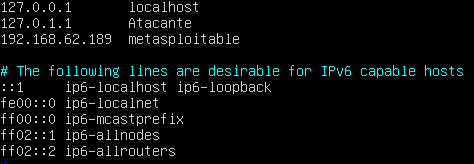
\includegraphics[width=0.5\textwidth]{./images/Atacante_dns_victima.png}
\caption{Atacante\_dns\_victima.}
\label{fig:nmap1}
\end{figure}

De esta forma, tenemos dos opciones para hacer referencia a la víctima. En la figura \ref{fig:nmap2} se observa el resultado de este escaneo simple fruto de cualquiera de estas dos opciones.

\begin{verbatim}
$ nmap 192.168.62.189
$ nmap metasploitable
\end{verbatim}

\begin{figure}[htbp]
\centering
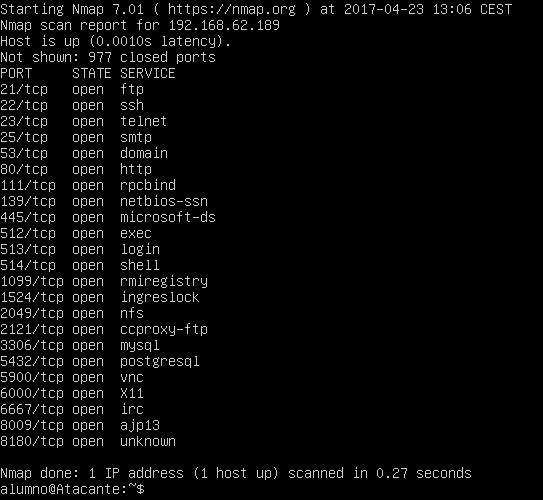
\includegraphics[width=0.8\textwidth]{./images/Atacante_nmap_simplescan.png}
\caption{Atacante\_nmap\_simplescan.}
\label{fig:nmap2}
\end{figure}

De forma un poco más elaborada, se puede ejecutar el escaneo de puertos haciendo uso de otras técnicas:

\begin{itemize}
  \item Mediante listado de equipos: \$ nmap 192.168.62.1 192.168.62.10 192.168.62.189
  \item Mediante subred: \$ nmap 192.168.62.0/24
  \item Mediante un fichero que almacene las IPs (o las expresiones de las mismas) a analizar: \$ nmap -iL hosts.txt, como muestra la figura \ref{fig:nmap3}.
\end{itemize}

\begin{figure}[htbp]
\centering
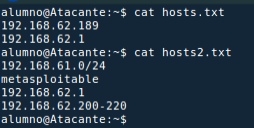
\includegraphics[width=0.4\textwidth]{./images/Atacante_nmapscan_filecomplex.png}
\caption{Atacante\_nmapscan\_filecomplex.}
\label{fig:nmap3}
\end{figure}

\subsubsection{NMAP con Metasploit}

También hemos de instalar Mestasploit para hacer uso de él: \url{https://github.com/rapid7/metasploit-framework/wiki/Nightly-Installers}. Una vez instalado, con \texttt{\$ msfconsole} inicializamos Metasploit y la base de datos asociada. \\

A continuación, realizamos un scanner básico de la red, almacenando el contenido en la base de datos interna y exportándolo completo de la misma a un fichero, para así analizarlo:

\begin{verbatim}
$ db_nmap -v -sV 192.168.62.0/24
$ db_export out_ejercicio1.txt
\end{verbatim}

Como muestra la figura \ref{fig:nmap4}, se observa que en dicho fichero encontramos el contenido del escaneo. Por un lado, podemos ver información del usuario que ha invocado el Metasploit. Seguidamente, tenemos el apartado que refiere a los hosts y servicios que se han encontrado en la dirección de subred que se le ha pasado al escaneo. Por último, podemos observar que el grueso del fichero son los módulos del Metasploit.

\begin{figure}[htbp]
\centering
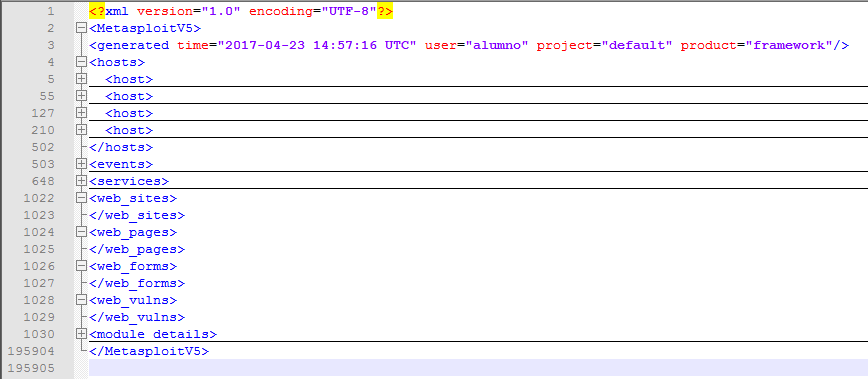
\includegraphics[width=1.0\textwidth]{./images/Atacante_scaner_y_BBDD.png}
\caption{Atacante\_scaner\_y\_BBDD.}
\label{fig:nmap4}
\end{figure}

\subsubsection{Wireshak: trazas}

A continuación mostramos algunas trazas obtenidas tras ejecutar ciertos comandos con NMAP.

\begin{itemize}
  \item \texttt{\$ nmap —scan-delay 1000ms -p 20-30 metasploitable}. En el host \texttt{metasploitable} se lanza un escaneo de puertos cada segundo a un puerto diferente entre los puertos 20 al 30, como muestra la figura \ref{fig:nmap5}. El fin principal de realizar un escaneo de puertos de esta forma es evitar ser detectado por la seguridad que pueda tener la subred.

  \begin{figure}[htbp]
  \centering
  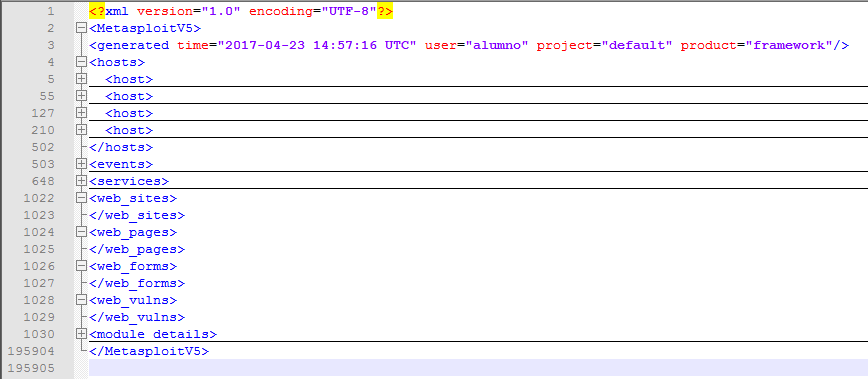
\includegraphics[width=1.0\textwidth]{./images/Atacante_scaner_y_BBDD.png}
  \caption{Atacante\_wireshar\_scaneo\_delay.}
  \label{fig:nmap5}
  \end{figure}

  \item \texttt{\$sudo nmap -sS -mtu 24 -p 80 metasploitable 192.168.62.102}. En el hots \texttt{metasploitable} y en la IP \texttt{192.168.62.102} se lanza un escaneo al puerto 80 con el bit SYN activado, como se muestra en la figura \ref{fig:nmap6} Lo que se hace es enviar un paquete SYN, como si se fuera a abrir una conexión real y después se espera una respuesta. Si se recibe un paquete SYN/ACK esto indica que el puerto está abierto, mientras que si se recibe un RST (reset) indica que no hay nada escuchando en el puerto. Si no se recibe ninguna respuesta después de realizar algunas retransmisiones o se recibe un ICMP entonces el puerto se marca como filtrado.

  \begin{figure}[htbp]
  \centering
  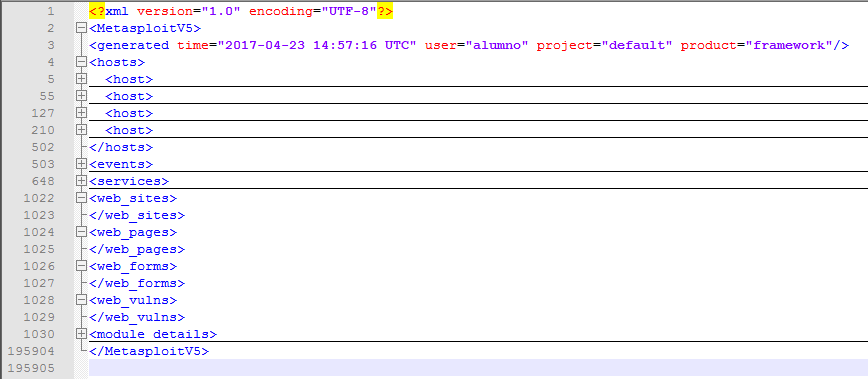
\includegraphics[width=1.0\textwidth]{./images/Atacante_scaner_y_BBDD.png}
  \caption{Atacante\_wireshar\_scaneo\_delay.}
  \label{fig:nmap6}
  \end{figure}

\end{itemize}

\end{document}
